%SPIEGARE SETUP E PROBLEMI (2 droni, haptic, problemi che ci sono in quest'ambito)
This chapter presents the architecture of the proposed two-drone framework and clarifies the main technical challenges addressed. 
\\Aerial robotics is a fundamental tool for operating in dangerous or degraded environments. UAVs are often used to keep human operators safe while performing non-destructive measurements on civil infrastructures. However, performing contact-based tasks requires a clear understanding of the workspace. When a drone approaches a structure, onboard First-Person View (FPV) cameras suffer from extreme occlusion and lack of depth perception. 
\\To overcome this limitation and maximize the human situational awareness, this thesis proposes an architecture centered around an active exocentric camera drone. In this setup, a second UAV acts as a target and performs the physical interaction with the environment. 
\\The observer drone must guarantee a stable video feed, avoiding any motion sickness for the human operator. At the same time, it must track a target drone whose trajectory is not known in advance. To solve this problem despite the underactuation of quadrotors, the system relies on a Non-linear Model Predictive Control (NMPC). This controller optimizes the camera framing and supports online POV adjustments commanded by the operator via a haptic device. 
\\Finally, the whole architecture is integrated with the standard PX4 firmware. Keeping the high-level logic connected to a known and tested flight stack provides reliable low-level stabilization and makes the transition to real hardware easier.

\section{Exocentric vision}
Using a standard onboard First-Person View (FPV) camera for physical interaction tasks presents some limitations. An egocentric perspective naturally compromises both the safety and the overall effectiveness of the mission.
When the inspection drone approaches a surface to make contact, the onboard camera ends up facing the wall from a very close distance. This completely blocks the Field of View (FOV). The human operator loses all environmental context, making it impossible to see surrounding obstacles or the actual position of the drone. An exocentric camera solves this simply by looking at the scene from the outside, keeping the full situational awareness intact.
\\Moreover, flying a drone toward a physical target using a flat, frontal 2D video feed makes it difficult to judge the remaining distance before impact. Depth perception is almost entirely lost. An observer drone tracking the operation from a lateral or isometric angle naturally restores this 3D spatial understanding, allowing the operator to clearly see the gap between the drone and the structure.
\begin{figure}[h!]
\centering
\begin{subfigure}[b]{0.49\textwidth}
    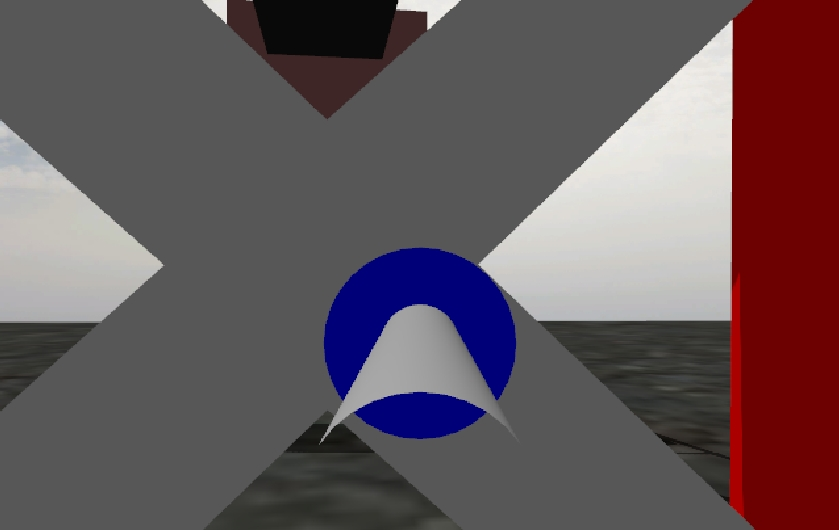
\includegraphics[width=\linewidth]{Immagini/Capitolo3/first_pov.jpg}
    \caption{Egocentric POV}
    \label{fig:first_pov_intro}
\end{subfigure}
\begin{subfigure}[b]{0.49\textwidth}
    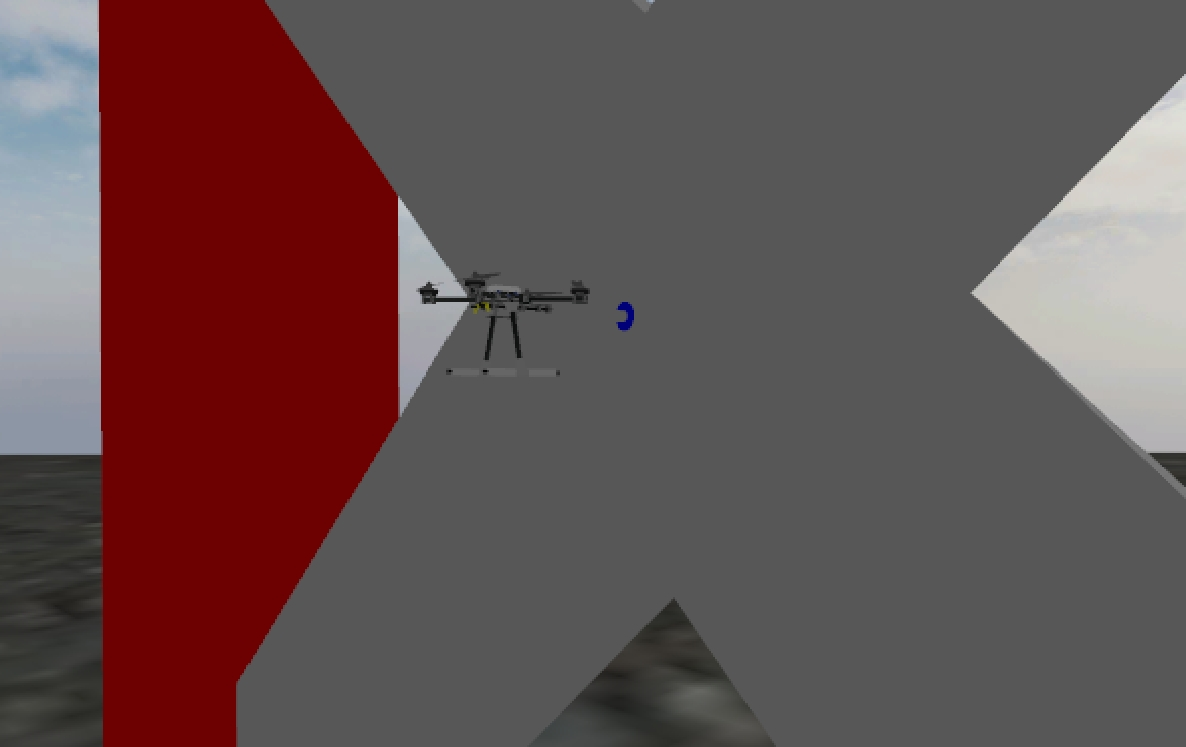
\includegraphics[width=\linewidth]{Immagini/Capitolo3/third_pov.jpg}
    \caption{Exocentric POV}
    \label{fig:third_pov_intro}
\end{subfigure}
\caption{Visual comparison between egocentric and exocentric views for bridge inspection task}
\end{figure}
\\Another major issue is the dynamic coupling of the quadrotor. Since standard quadrotors are underactuated, they must tilt to move or apply forces against a wall. If the camera is rigidly attached to the inspection drone, it will shake with every single pitch, roll, or contact vibration. The resulting video feed becomes chaotic, degrading the inspection quality and easily causing motion sickness for the operator. By using an independent observer drone, the visual task is completely decoupled from the physical one. The MPC can then focus entirely on planning a smooth and stable camera trajectory, isolating the operator from the rough dynamics the contact drone has to face.
\section{Shared control}
A fully autonomous operation is often unfeasible in unstructured environments. The human operator must be able to intervene during the mission. For this reason, a haptic device is integrated into the control loop. 
\\The operator uses the haptic interface for two main purposes. The first one is to dynamically change the Point of View (POV) of the observer drone. This intervention is necessary in case of sudden occlusions, unexpected obstacles, or a general loss of situational awareness. The operator can move the external camera to find a better angle without interrupting the tracking task. 
\begin{figure}
    \centering
    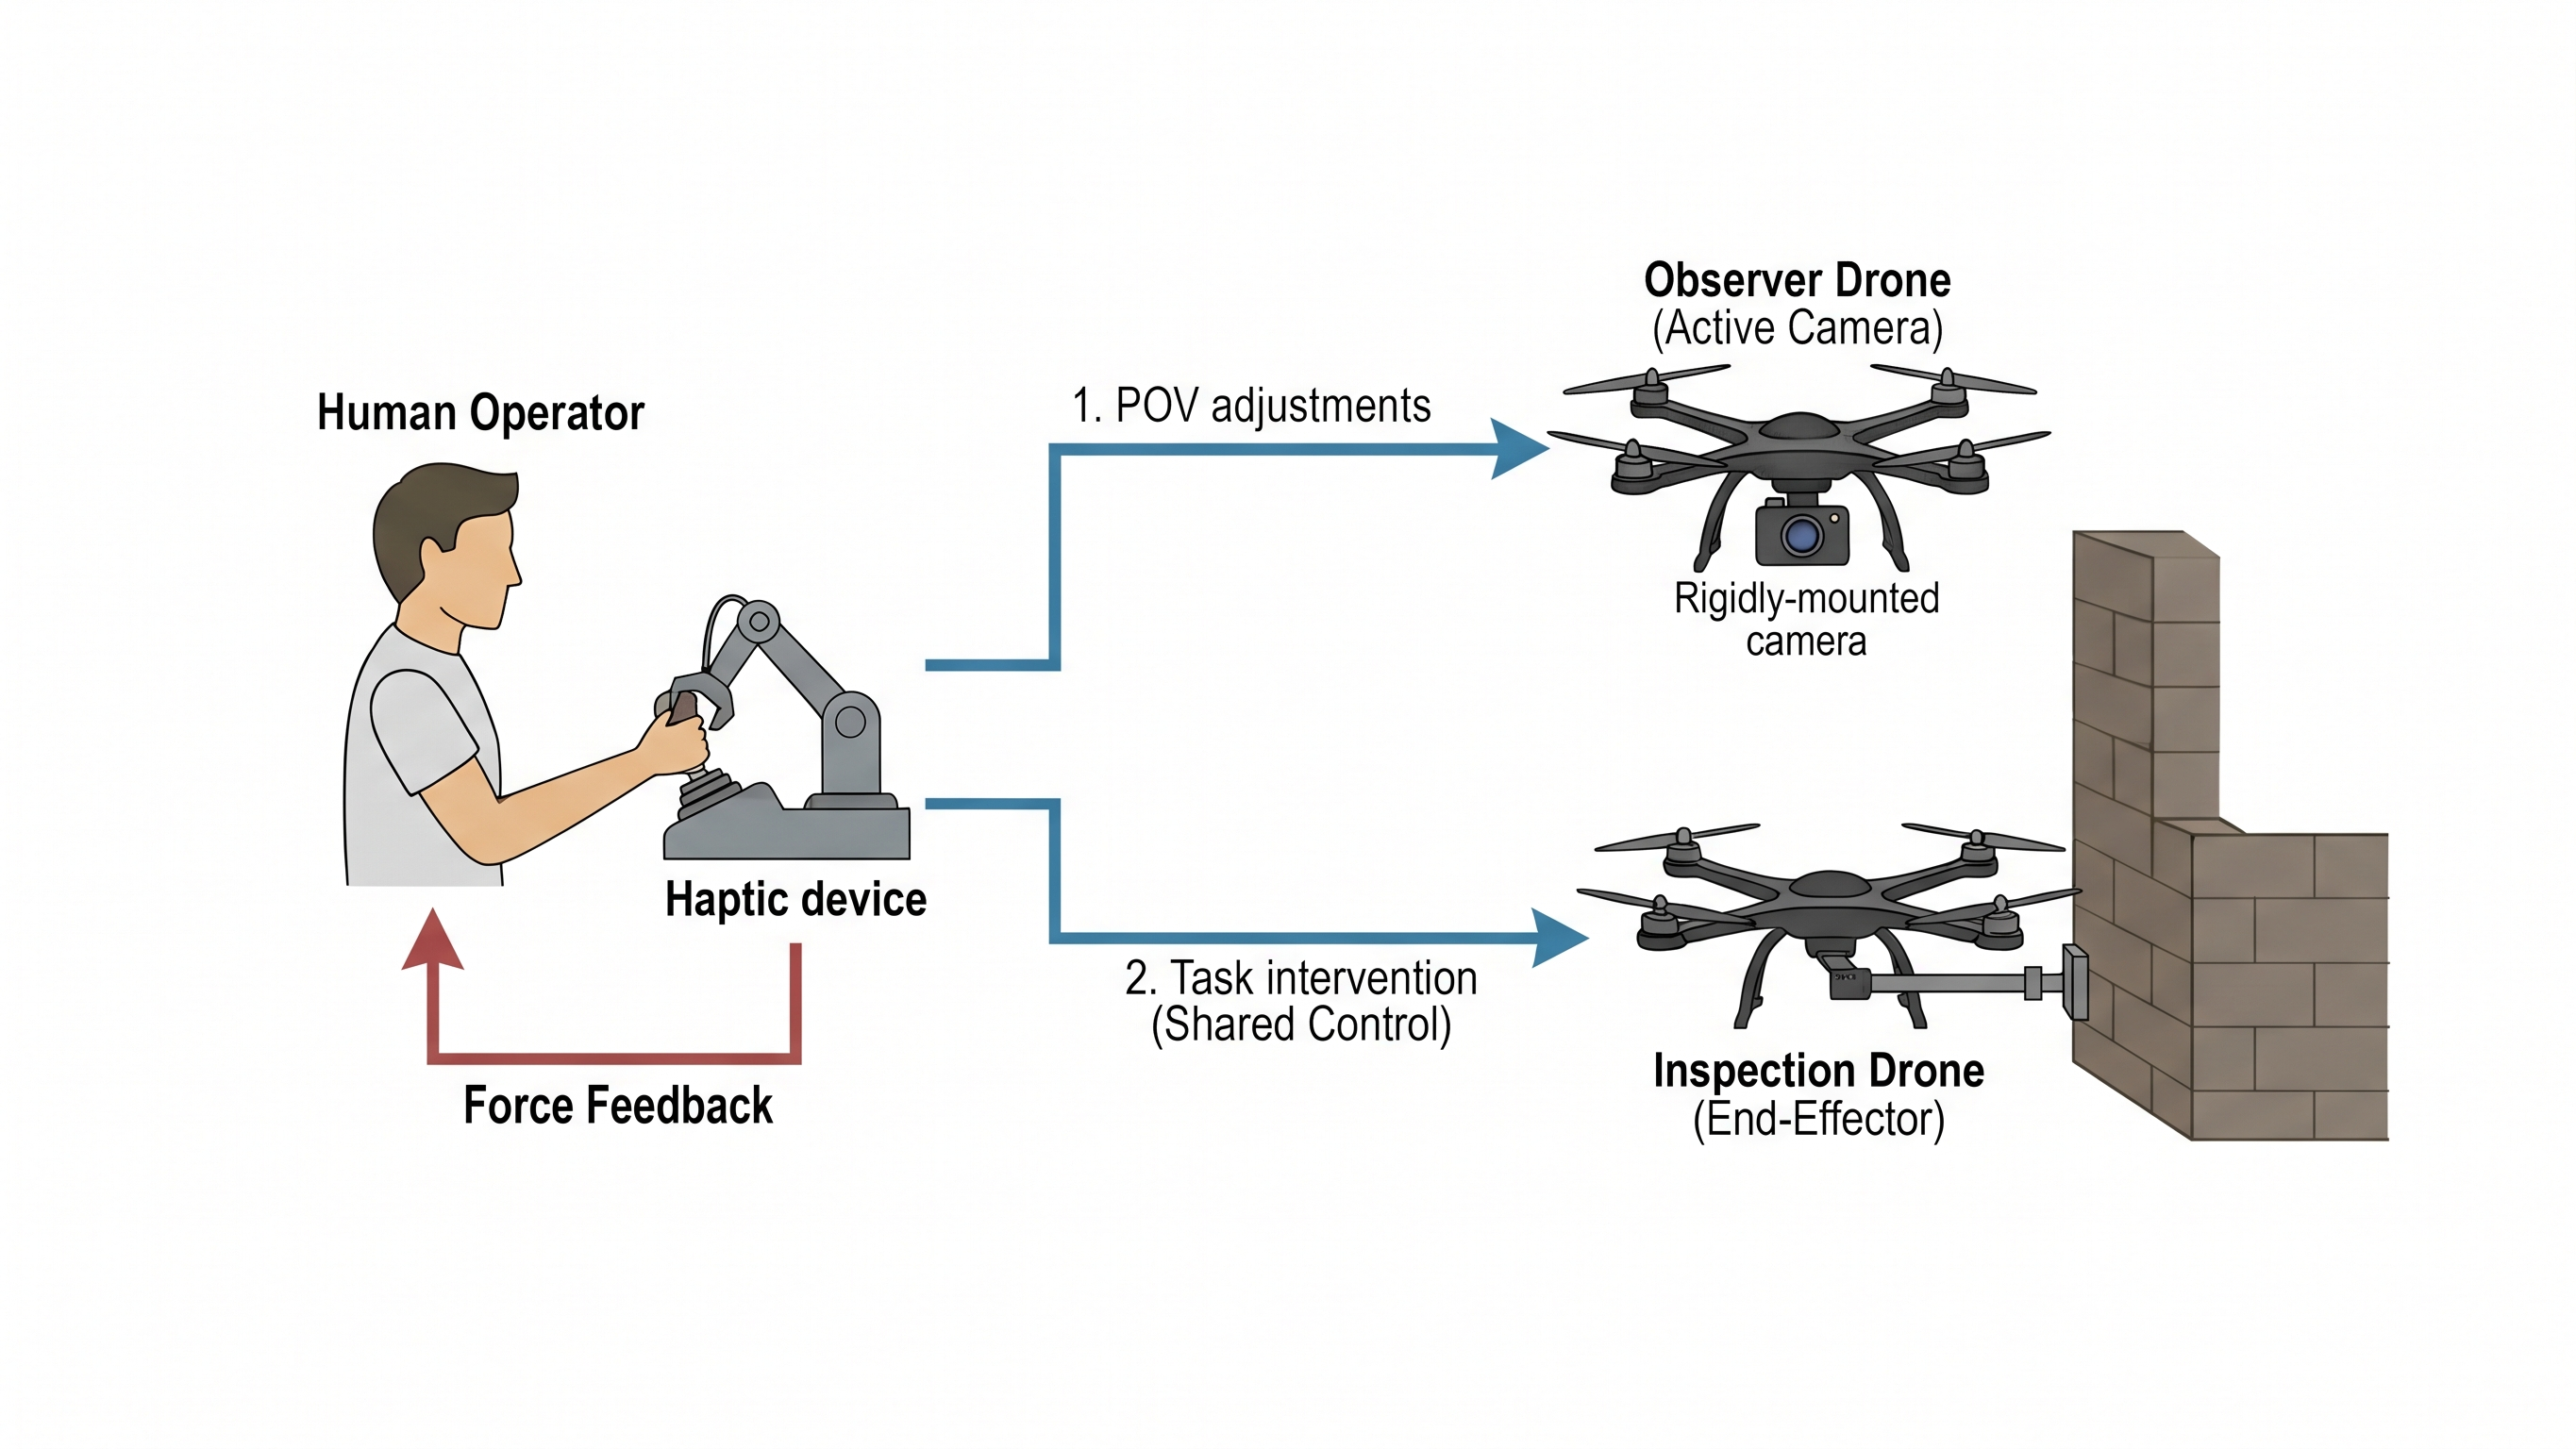
\includegraphics[width=\linewidth]{Immagini/Capitolo3/Shared Control.jpeg}
    \caption{Bilateral teleoperation illustration}
    \label{fig:shared_control_intro}
\end{figure}
\\The second purpose is to take direct control of the inspection drone. During the interaction phase of the mission, the operator guides the platform to perform the non-destructive measurements in a controlled way. In this case, the human decision-making is combined with the low-level admittance filter to maintain a stable contact with the wall.
\\Furthermore, the haptic device provides physical feedback to the user; for this reason we speak about \textit{bilateral teleoperation}. The mathematical limits of the camera field of view and the safety distances are translated into repulsive forces. This physical sensation prevents the operator from losing the target or crashing the drones.
\section{Contact inspection}
The execution of physical contact tasks with a multi-rotor platform introduces complexities with respect to standard free-flight navigation. When the inspection drone physically interacts with a rigid surface, such as a bridge pillar, it experiences environmental reaction forces. If the UAV is governed by a standard position controller, it will interpret the physical wall simply as a persistent position error, keeping pushing inside it. This mismatch causes the controller to aggressively increase its control input in an attempt to reach the unfeasible reference inside the wall, leading to violent inclination, actuator saturation, and potential crashes.
\begin{figure}[h!]
    \centering
    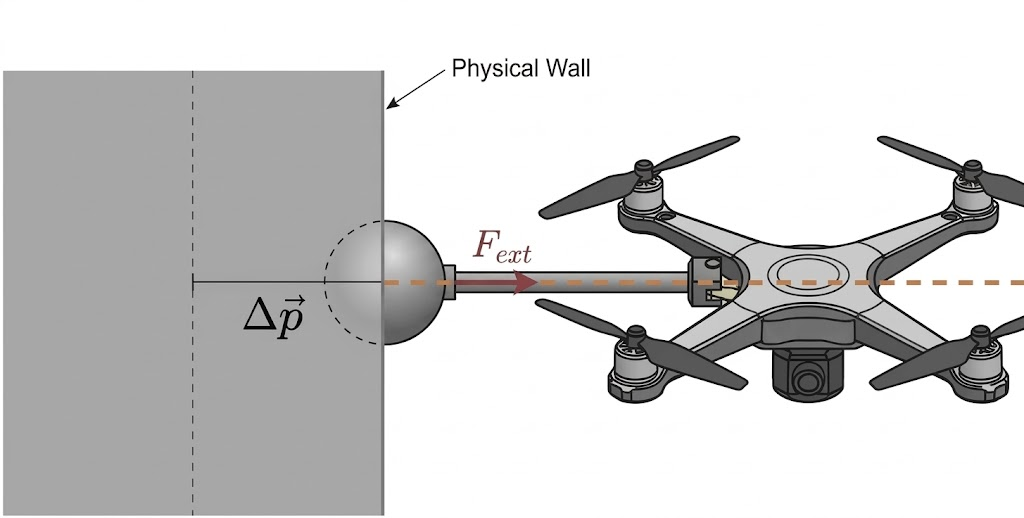
\includegraphics[width=0.5\linewidth]{Immagini/Capitolo3/Drone_interaction.jpeg}
    \caption{Drone interacting with environment; position goal behind the wall}
    \label{fig:interaction_intro}
\end{figure}
To safely manage this interaction, the architecture implements an admittance filter that makes the drone compliant with the environment, conceptually acting as a virtual spring-damper system. Instead of rigidly tracking a static geometric setpoint, the admittance framework translates the external contact forces into a real-time modification of the desired trajectory. When the drone pushes against the surface, the filter acts, safely adjusting the position reference backwards to maintain a stable contact. 
\\Even if admittance control ensures the low-level physical stability of the inspection drone, guiding the UAV to the exact target point remains a very delicate operation. This is where the exocentric vision framework becomes fundamental. By delegating the local contact safety to the autonomous admittance filter, the target drone's behavior becomes stable. This allows the human operator to focus entirely on the high-level contact maneuver and mission monitoring through the optimal and adapted 3D viewpoint continuously provided by the observer drone.

\section{A system architecture overview}
The overall system is built on a distributed software architecture using ROS2. This middleware acts as a bridge, smoothly connecting the high-level control algorithms with the low-level flight firmware. On the hardware side, both quadrotors rely on the PX4 autopilot, which manages essential tasks like state estimation and motor mixing.
\begin{figure}[htbp]
    \centering
    \resizebox{\textwidth}{!}{%
    \begin{tikzpicture}[
        % Definizione degli stili
        human/.style={rectangle, draw=black, thick, fill=gray!10, text centered, rounded corners, minimum height=1.2cm, minimum width=2.5cm, font=\sffamily\small},
        rosnode/.style={rectangle, draw=blue!80!black, thick, fill=blue!5, text centered, rounded corners, minimum height=1.2cm, minimum width=3cm, font=\sffamily\small, align=center},
        px4/.style={rectangle, draw=orange!80!black, thick, fill=orange!10, text centered, rounded corners, minimum height=1.2cm, minimum width=3cm, font=\sffamily\small, align=center},
        hardware/.style={rectangle, draw=green!60!black, thick, fill=green!5, text centered, minimum height=1.2cm, minimum width=2.5cm, font=\sffamily\small, align=center},
        arrow/.style={-{Stealth[scale=1.2]}, thick},
        dashed_arrow/.style={-{Stealth[scale=1.2]}, thick, dashed},
        groupbox/.style={rectangle, draw=#1, dashed, thick, inner sep=0.4cm, rounded corners},
        labeltext/.style={font=\sffamily\scriptsize, fill=white, inner sep=2pt, align=center}
    ]

    % ================== POSIZIONAMENTO DEI NODI A GRIGLIA ==================
    % Colonna 1 (x=0): Interazione Umana
    \node[human] at (0, 2) (operator) {Human\\Operator};
    \node[hardware] at (0, 0) (haptic) {Haptic Interface\\(Novint Falcon)};

    % Colonna 2 (x=4): Nodi ROS 2 (Supervisione e Teleoperazione)
    \node[rosnode] at (4, 2) (supervisor) {Mission Supervisor\\(FSM)};
    \node[rosnode] at (4, 0) (teleop) {Haptic \& Teleop\\Node (APF)};

    % Colonna 3 (x=8.5): Nodi ROS 2 (Algoritmi di Controllo)
    \node[rosnode] at (9, 2) (mpc) {Obs UAV\\NMPC Node};
    \node[rosnode] at (9, 0) (admittance) {Insp UAV\\Adm Filter};

    % Colonna 4 (x=13): Firmware Basso Livello (PX4)
    \node[px4] at (13, 2) (px4_obs) {PX4 Autopilot\\};
    \node[px4] at (13, 0) (px4_ins) {PX4 Autopilot\\(Position PID)};

    % Colonna 5 (x=17): Piattaforme Fisiche
    \node[hardware] at (17, 2) (drone_obs) {Observer\\UAV};
    \node[hardware] at (17, 0) (drone_ins) {Inspection\\UAV};

    % Sensori Addizionali ed Estimatore
    \node[hardware] at (17, -2) (ft_sensor) {F/T Sensor};
    \node[px4, minimum width=4cm] at (13, -4) (estimator) {State Estimation\\(OptiTrack / PX4 EKF2)};

    % ================== BACKGROUND BOXES ==================
    \begin{scope}[on background layer]
        % Box ROS 2 High-Level
        \node[groupbox=blue!80!black, fit=(supervisor) (teleop) (mpc) (admittance)] (rosbox) {};
        \node[above left, font=\sffamily\bfseries\color{blue!80!black}] at (rosbox.north east) {ROS 2 High-Level Network};

        % Box PX4 Low-Level
        \node[groupbox=orange!80!black, fit=(px4_obs) (px4_ins) (estimator)] (px4box) {};
        \node[above left, font=\sffamily\bfseries\color{orange!80!black}] at (px4box.north east) {Low-Level Firmware};
    \end{scope}

    % ================== COLLEGAMENTI E FRECCE ==================
    
    % 1. Human <-> Haptic
    \draw[<->, thick] (operator) -- node[right, labeltext] {Haptic Feedback\\\& Motion Input} (haptic);

    % 2. Haptic <-> Teleop (Frecce sfalsate per evitare sovrapposizioni)
    \draw[arrow] ([yshift=2mm]haptic.east) -- node[above, labeltext] {$p_h, \dot{p}_h$} ([yshift=2mm]teleop.west);
    \draw[arrow] ([yshift=-2mm]teleop.west) -- node[below, labeltext] {Forces} ([yshift=-2mm]haptic.east);

    % 3. Flusso Teleoperazione verso i Controllori
    % Teleop -> MPC (Deviato in alto per non toccare Supervisor)
    \draw[arrow] ([yshift=2mm]teleop.east) -| (6.0, 1.8) -- node[above, labeltext] {$y_{ref}$} ([yshift=-2mm]mpc.west);
    % Teleop -> Admittance (Linea dritta orizzontale)
    \draw[dashed_arrow] ([yshift=-2mm]teleop.east) -- node[below, labeltext] {Shared\\Control} ([yshift=-2mm]admittance.west);

    % 4. Comandi del Supervisor
    \draw[dashed_arrow] (supervisor.south) -- node[right, labeltext] {State/FSM} (teleop.north);
    \draw[dashed_arrow] (supervisor.east) -- node[above, labeltext] {State/FSM} (mpc.west);
    % Supervisor -> Admittance (Scende e gira verso destra)
    \draw[dashed_arrow] ([yshift=-2mm]supervisor.east) -| (6.5, 0.2) -- node[above of=2mm, labeltext] {State/FSM} ([yshift=2mm]admittance.west);

    % 5. Interfacciamento ROS 2 -> PX4
    \draw[arrow] (mpc.east) -- node[above, labeltext] {$T, \tau$} (px4_obs.west);
    \draw[arrow] (admittance.east) -- node[above, labeltext] {$x_c, v_c$} (px4_ins.west);

    % 6. PX4 -> Output Fisico
    \draw[arrow] (px4_obs.east) -- node[above, labeltext] {PWM} (drone_obs.west);
    \draw[arrow] (px4_ins.east) -- node[above, labeltext] {PWM} (drone_ins.west);

    % 7. Sensore di Forza
    \draw[arrow] (drone_ins.south) -- (ft_sensor.north);
    % FT Sensor -> Admittance (Passa a un'altezza sicura y=-2)
    \draw[arrow] (ft_sensor.west) -- node[above, labeltext] {Contact Force $F_{ext}$} (9, -2) -- (admittance.south);

    % 8. Flusso Telemetria (Droni -> Estimatore, passando esternamente a destra)
    \draw[arrow, dashed] (drone_obs.east) -| ++(1.0, -6) |- node[below near start, labeltext] {Telemetry} ([yshift=2mm]estimator.east);
    \draw[arrow, dashed] (drone_ins.east) -| ++(0.6, -4) |- ([yshift=-2mm]estimator.east);

    % 9. Bus di Feedback dello Stato (Estimatore -> Nodi ROS 2)
    % Linea orizzontale principale in basso
    \draw[thick] (estimator.west) -- node[below, labeltext] {State Feedback $x$} (4.0, -4);
    % Diramazioni verso l'alto
    \draw[arrow] (4.0, -4) -- (teleop.south);
    \draw[arrow] (8.0, -4) -- ([xshift=-10mm]mpc.south);
    \draw[arrow] (8.5, -4) -- ([xshift=-5mm]admittance.south);

    \end{tikzpicture}
    } % Fine resizebox
    \caption{Block diagram of the overall system architecture. The ROS 2 block computes "high-level" commands, generating direct thrust and torques for the observer drone (via NMPC) and compliant position setpoints for the inspection drone (via Admittance Filter). The PX4 flight stack executes low-level actuation and state estimation.}
    \label{fig:system_architecture}
\end{figure}
\justify
The brain of the exocentric observation resides in the real-time Model Predictive Control (MPC) node governing the observer drone. This continuously processes the dynamic state of the inspection UAV to actively frame it, while integrating high-level viewpoint adjustments from the human operator. By solving an optimization problem on the fly, the MPC finds the best possible tracking path while strictly respecting the drone's physical limits. To maximize efficiency, the MPC bypasses traditional cascaded position planners, computing and sending thrust and torque commands directly to the PX4 offboard control module, acting as controller and planner at the same time.
\\A key element of this human-in-the-loop setup is the haptic interface, which creates a two-way communication channel between the operator and the robotic team. When the user moves the device, these inputs are translated into velocity commands that update the desired PoV. Simultaneously, the operator receives continuous physical feedback calculated using artificial potential fields method. Essentially, it physically guides the user to stay within safe distances and keeps the target well inside the camera's field of view.
\\The inspection drone uses a different control strategy, specifically thought for physical interaction. Its planner generates standard position targets, which are then continuously adjusted by the admittance filter based on the forces sensed from the environment. These compliant targets are fed into the standard PX4 position controller. This dual approach perfectly balances the mission requirements: reactive and optimal visual tracking from the observer drone, paired with safe and stable contact from the inspection drone.

\section{Mission description}
The cooperative inspection mission is performed as a Finite State Machine (FSM), ensuring safety and reliability at each step of the operation. The mission is divided into distinct operational phases, managed by a central supervisor node and the state transitions are governed by autonomous safety checks coupled with human-in-the-loop confirmations via keyboard input. Figure \ref{fig:fsm_mission} illustrates the state transitions governing the entire system.

% Diagramma FSM
\begin{figure}[htbp]
    \centering
    \resizebox{\textwidth}{!}{%
    \begin{tikzpicture}[
        node distance=1.6cm and 1.8cm,
        state/.style={rectangle, rounded corners, draw=black, thick, fill=blue!5, minimum width=2.8cm, minimum height=1.2cm, text centered, font=\sffamily\small, align=center},
        arrow/.style={-{Stealth[scale=1.2]}, thick},
        phasebox/.style={rectangle, draw=#1, dashed, thick, inner sep=1.2em, rounded corners},
        labeltext/.style={font=\sffamily\scriptsize\itshape, align=center, text width=2.5cm}
    ]

    % --- ROW 1: PHASE 1 ---
    \node[state] (wait_ekf) {WAIT EKF};
    \node[state, right=of wait_ekf] (wait_takeoff) {WAIT TAKEOFF};
    \node[state, right=of wait_takeoff] (arm) {ARM OFFBOARD};
    \node[state, right=of arm] (monitor) {TAKEOFF MONITOR};

    % --- ROW 2: PHASE 2 & 3 (R-to-L flow to save space) ---
    \node[state, below=2.5cm of monitor] (hovering) {HOVERING};
    \node[state, left=3cm of hovering] (approach) {APPROACH};
    \node[state, left=4cm of approach] (interaction) {INTERACTION};

    % --- ROW 3: PHASE 4 (L-to-R flow) ---
    \node[state, below=3cm of interaction] (detachment) {DETACHMENT};
    \node[state, right=of detachment] (return_home) {RETURN HOME};
    \node[state, right=of return_home] (landing) {LANDING};
    \node[state, right=of landing] (complete) {MISSION COMPLETE};

    % --- EMERGENCY BOX ---
    \node[state, fill=red!10, draw=red, thick, above right=0.8cm and -1.0cm of monitor] (emergency) {EMERGENCY};
    \node[font=\sffamily\scriptsize\color{red}, left=0.5cm of emergency, align=right] (any) {Any state\\("stop" cmd or Fail)};
    \draw[arrow, red, dashed] (any) -- (emergency);

    % --- PHASE BACKGROUND BOXES ---
    \begin{scope}[on background layer]
        % Phase 1
        \node[phasebox=blue, fit=(wait_ekf) (monitor)] (phase1) {};
        \node[above right, font=\sffamily\bfseries\color{blue}] at (phase1.north west) {Phase 1: Initialization \& Take-off};

        % Phase 2
        \node[phasebox=orange, fit=(hovering) (approach)] (phase2) {};
        \node[above left, font=\sffamily\bfseries\color{orange}] at (phase2.north east) {Phase 2: Navigation \& Approach};

        % Phase 3
        \node[phasebox=green!60!black, fit=(interaction)] (phase3) {};
        \node[above right, font=\sffamily\bfseries\color{green!60!black}] at (phase3.north west) {Phase 3: Contact Inspection};

        % Phase 4
        \node[phasebox=purple, fit=(detachment) (complete)] (phase4) {};
        \node[above right, font=\sffamily\bfseries\color{purple}] at (phase4.north west) {Phase 4: Detachment \& Landing};
    \end{scope}

    % --- ARROWS & TRANSITIONS ---
    % Phase 1
    \draw[arrow] (wait_ekf) -- node[above, labeltext] {EKF \\converged} (wait_takeoff);
    \draw[arrow] (wait_takeoff) -- node[above, labeltext] {Takeoff\\authorization} (arm);
    \draw[arrow] (arm) -- node[above, labeltext] {Armed \&\\Offboard} (monitor);
    
    % Phase 1 -> 2
    \draw[arrow] (monitor) -- node[right, labeltext, yshift=2mm] {Altitude reached +\\Operator OK} (hovering);
    
    % Phase 2
    \draw[arrow] (hovering) -- node[above, labeltext] {Hovering reached +\\Operator OK} (approach);
    
    % Phase 2 -> 3
    \draw[arrow] (approach) -- node[above, labeltext] {Approach pose reached +\\Operator OK} (interaction);
    
    % Phase 3 -> 4
    \draw[arrow] (interaction) -- node[right, labeltext, yshift=2mm] {Inspection Done +\\Operator OK} (detachment);
    
    % Phase 4
    \draw[arrow] (detachment) -- node[above, labeltext] {Detachment completed +\\Operator OK} (return_home);
    \draw[arrow] (return_home) -- node[above, labeltext] {Home \\reached +\\Operator OK} (landing);
    \draw[arrow] (landing) -- node[above, labeltext] {Drones\\disarmed} (complete);

    \end{tikzpicture}
    } % Fine resizebox
    \caption{Finite State Machine (FSM) representing the sequential phases of the cooperative mission. State transitions are governed by autonomous checks and human-in-the-loop confirmations managed by the supervisor node.}
    \label{fig:fsm_mission}
\end{figure}

\begin{itemize}
    \item \textbf{Phase 1: Initialization and Take-off.} The mission begins with the supervisor node awaiting the full Extended Kalman Filter (EKF) convergence for both drones (\texttt{WAIT EKF}). Upon human confirmation, the system transitions to \texttt{WAIT TAKEOFF}, verifying the MPC readiness before autonomously arming and switching both vehicles to offboard control mode (\texttt{ARM OFFBOARD}). Finally, both UAVs take off and hover at a predefined safety altitude, monitored continuously until reached (\texttt{TAKEOFF MONITOR}). 
    \item \textbf{Phase 2: Navigation and Approach.} Once altitude is reached and the operator confirms, the system moves to the \texttt{HOVERING} state. The Inspection Drone (Drone 2) holds its starting coordinate, while the Camera Drone initiates the visual tracking via MPC, framing Drone 2 centrally. Following another operator confirmation, Obseerved Drone autonomously navigates towards the target inspection area (e.g., a position $2\text{ m}$ away from a bridge pillar) and aligns its yaw (\texttt{APPROACH}). Throughout this phase, Drone 1 actively maintains the target in the center of its Field of View (FOV).
    \item \textbf{Phase 3: Contact Inspection and Shared Control.} After operator confirm, the system transitions into \texttt{INTERACTION}. Drone 2 advances to make physical contact with the structure. Concurrently, the supervisor commands the MPC of Drone 1 to adopt a closer and decentered Point of View (PoV) (e.g., observing Drone 2 in the bottom-right corner of the FOV), providing optimal visual context for the task. In this phase the human operator uses haptic interface, allowing for fine-grained manual scanning.
    \item \textbf{Phase 4: Detachment and Landing.} When the inspection is concluded, an operator command triggers the \texttt{DETACHMENT} state. Drone 2 safely detaches from the wall, retreating by a predetermined distance ($1\text{ m}$), while Drone 1 widens its tracking radius to $2.0\text{ m}$, to have a larger view, while preserving the decentered PoV. Upon further clearance, the vehicles retreat to the \texttt{RETURN HOME} state: Drone 2 navigates back to its initial take-off location, and Drone 1 restores a centered PoV. Finally, the supervisor commands \texttt{LANDING}, safely bringing both drones to the ground until disarmed (\texttt{MISSION COMPLETE}). At any point during the mission, an operator ``stop" command or an offboard/arming failure triggers an immediate \texttt{EMERGENCY} state, enforcing a prompt landing.
\end{itemize}